\documentclass{beamer}
\usepackage[utf8]{inputenc}
%\usepackage[russian]{babel}
\usepackage{amsmath,mathrsfs}
\usepackage{graphicx, epsfig}
\usetheme{Warsaw}%{Singapore}%{Warsaw}%{Warsaw}%{Darmstadt}
\usecolortheme{sidebartab}
\usepackage{graphicx}
\definecolor{beamer@blendedblue}{RGB}{15,120,80}
%----------------------------------------------------------------------------------------------------------
\title[\hbox to 56mm{TOUCH  \hfill\insertframenumber\,/\,\inserttotalframenumber}]
{TOUCH: In-Memory Spatial Join by Hierarchical Data-Oriented Partitioning}
\author[A.\,Logins]{\large \\A.\, Logins}
\institute{\large
Moscow Institute of Physics and Technology\par
Skolkovo Institute of Science and Technology}

\date{\footnotesize{\emph{Course:} Machine Learning and Data Analysis\par (Strijov's practice)/Group 174, 2014 Fall}}
%----------------------------------------------------------------------------------------------------------
\begin{document}
%----------------------------------------------------------------------------------------------------------
\begin{frame}
%\thispagestyle{empty}
\titlepage
\end{frame}
%-----------------------------------------------------------------------------------------------------
\begin{frame}{Goal of research}
\begin{block}{Motivation}
\begin{itemize}
\item Finding close objects with complex shape in space from large datasets can be a hard problem, that requires effective indexing of data and search algorithms
\item State-of-art solutions are restrained by taking into consideration time for reading data from main memory (hard disc)
\end{itemize}
+ Recent research TOUCH is designed for in-memory join and performs much faster\\
- It suffers from strong unbalance inside data structure used for indexing, which leads to extreme dependency from data distribution and prevents from effective parallelization.\\
Fixing the design of TOUCH would give new super-fast spatial join algorithm.
\end{block}
\end{frame}
%----------------------------------------------------------------------------------------------------------
\begin{frame}{Problem of spatial join}
Given the parameter $\epsilon$ and two datasets of spatial objects $A$ and $B$ find all $a\in A$ and $b \in B$ such that minimum distance between them is less than $\epsilon$.
\begin{figure}[p]
    \centering
    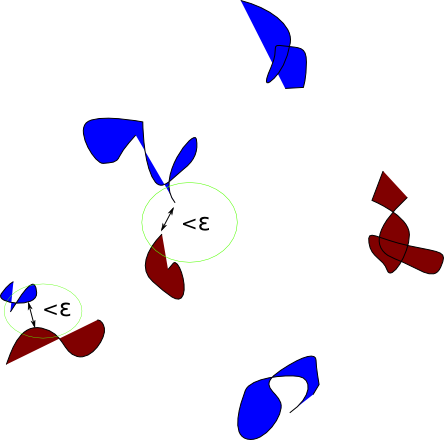
\includegraphics[width=0.4\textwidth]{Images/spjoin.png}
\end{figure}
\end{frame}
%----------------------------------------------------------------------------------------------------------
\begin{frame}{Solution : Building step}
First step: building spatial index structure (R-tree) using objects of first type
\begin{figure}[p]
    \centering
    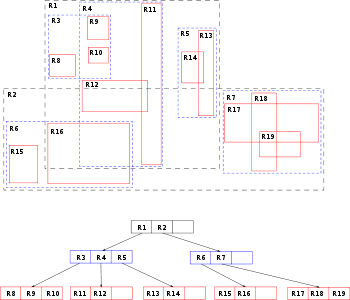
\includegraphics[width=0.6\textwidth]{Images/3dRtree.png}
\end{figure}
\end{frame}
\begin{frame}{Solution : Assignment step}
Second step: assigning objects of second type to the nodes of the tree
\begin{figure}[p]
    \centering
    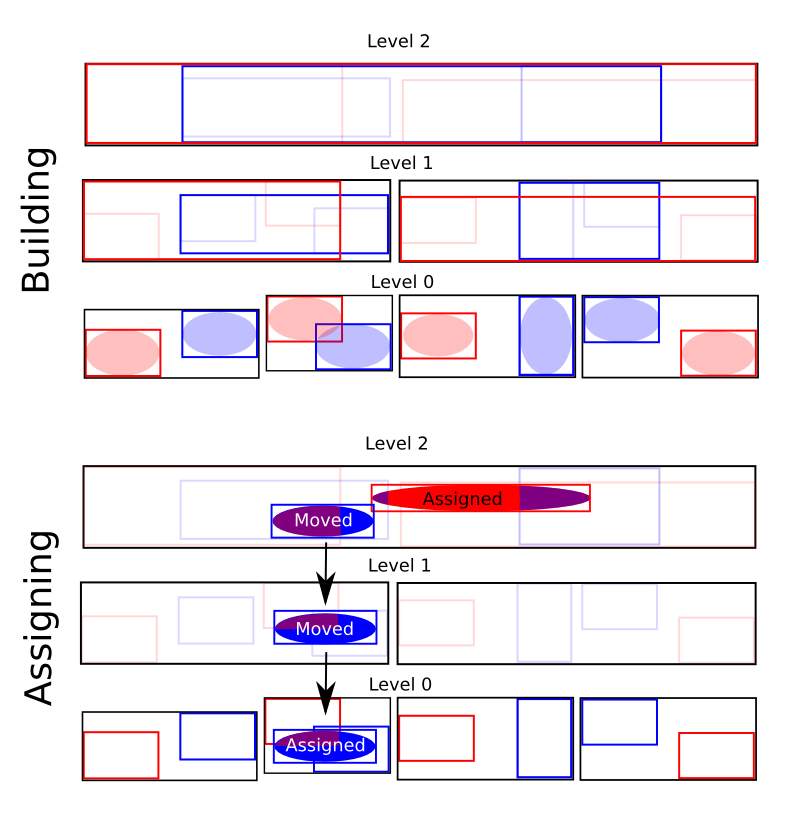
\includegraphics[width=0.6\textwidth]{Images/cTOUCHexplain.png}
\end{figure}
\end{frame}
\begin{frame}{Solution : Assignment step (variations)}
Second step: variations
\begin{itemize}
\item (dTOUCH) do not assign higher than some level. Build another tree for skipped objects
\item (cTOUCH) build initial index using both data types simultaneously. Assign objects that were cut from leaf nodes. Dynamically fix MBRs
\item (reTOUCH) after usual assignment step remove all objects of first dataset, fix MBRs (build new tree using old skeleton) of left objects and reassign removed objects. 
\item (rereTOUCH) repeat one more reTOUCH iteration
\end{itemize}
\end{frame}
\begin{frame}{Solution : Joining step}
Third step: Joining step, checking two buckets of objects using their arbitrary spatial shape. \\
Using either Nested Loop or Spatial Grid Hash
\begin{figure}[p]
    \centering
    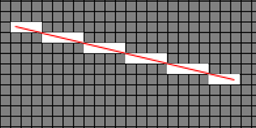
\includegraphics[width=0.6\textwidth]{Images/line.png}
\end{figure}
\end{frame}
%----------------------------------------------------------------------------------------------------------
\begin{frame}{Computational experiment : Filtering A}
\begin{figure}[p]
    \centering
    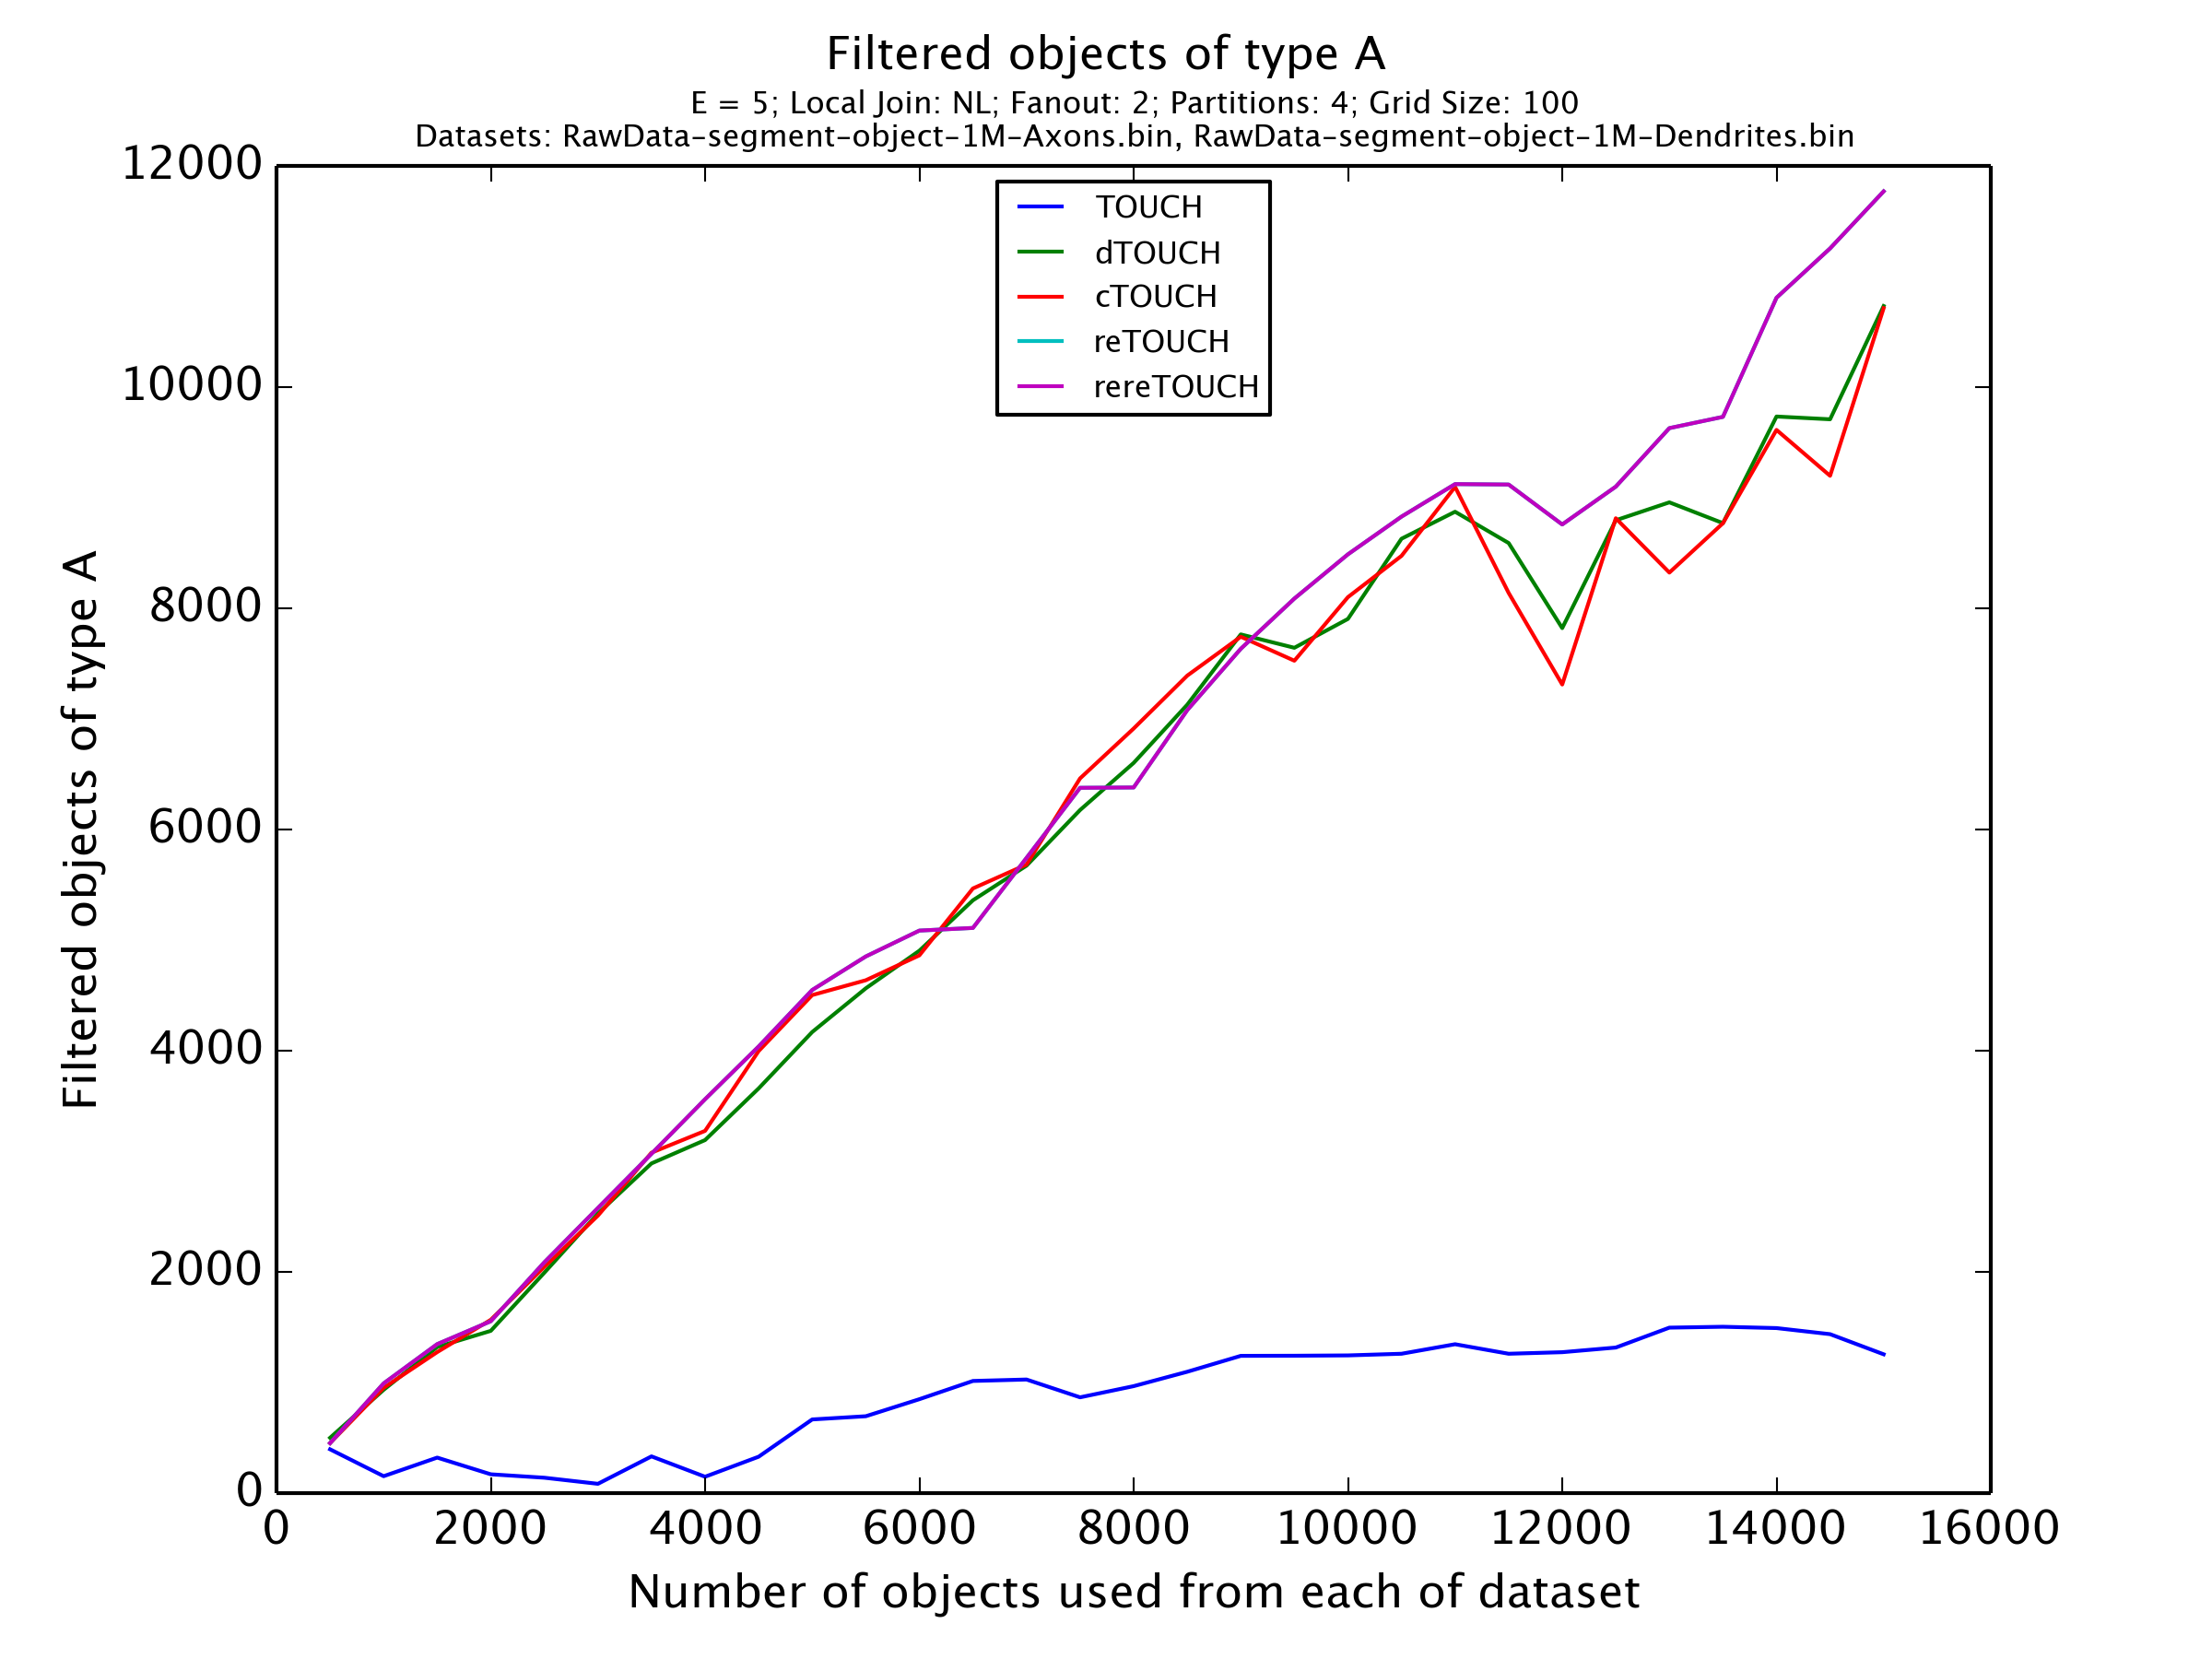
\includegraphics[width=0.8\textwidth]{Images/pic16.png}
\end{figure}
\end{frame}
\begin{frame}{Computational experiment : Filtering B}
\begin{figure}[p]
    \centering
    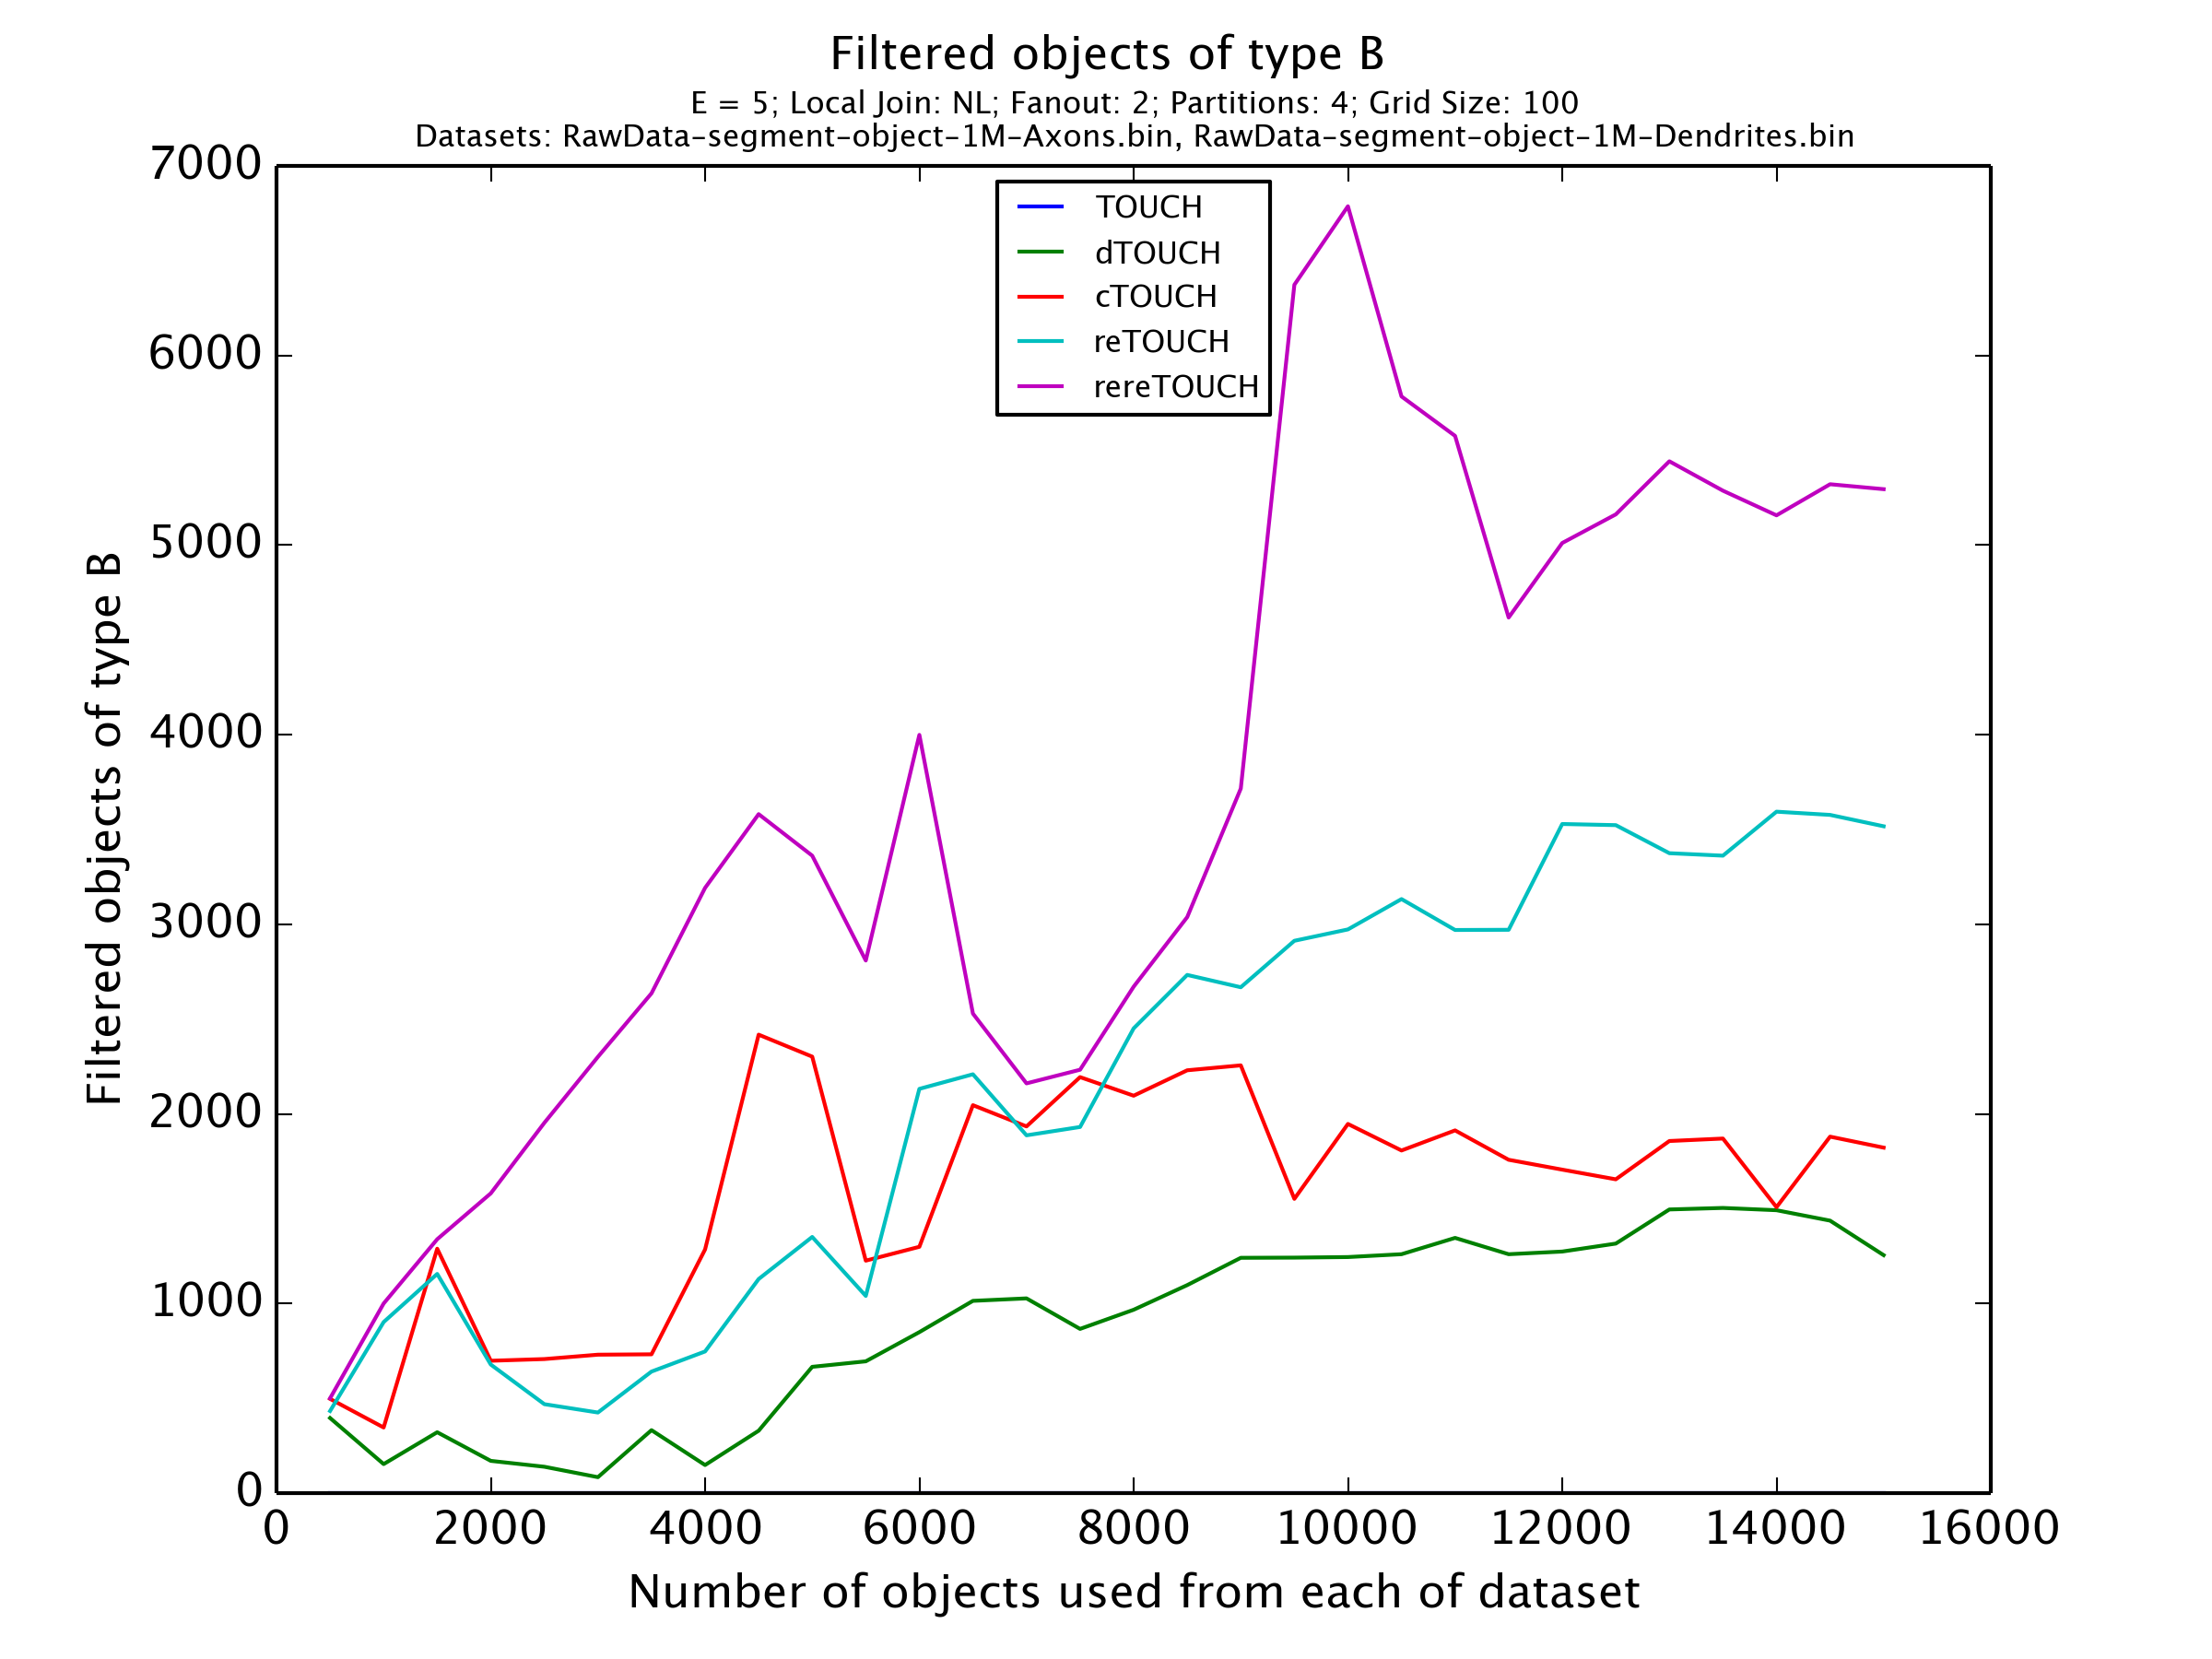
\includegraphics[width=0.8\textwidth]{Images/pic17.png}
\end{figure}
\end{frame}
\begin{frame}{Computational experiment : Assignment time}
\begin{figure}[p]
    \centering
    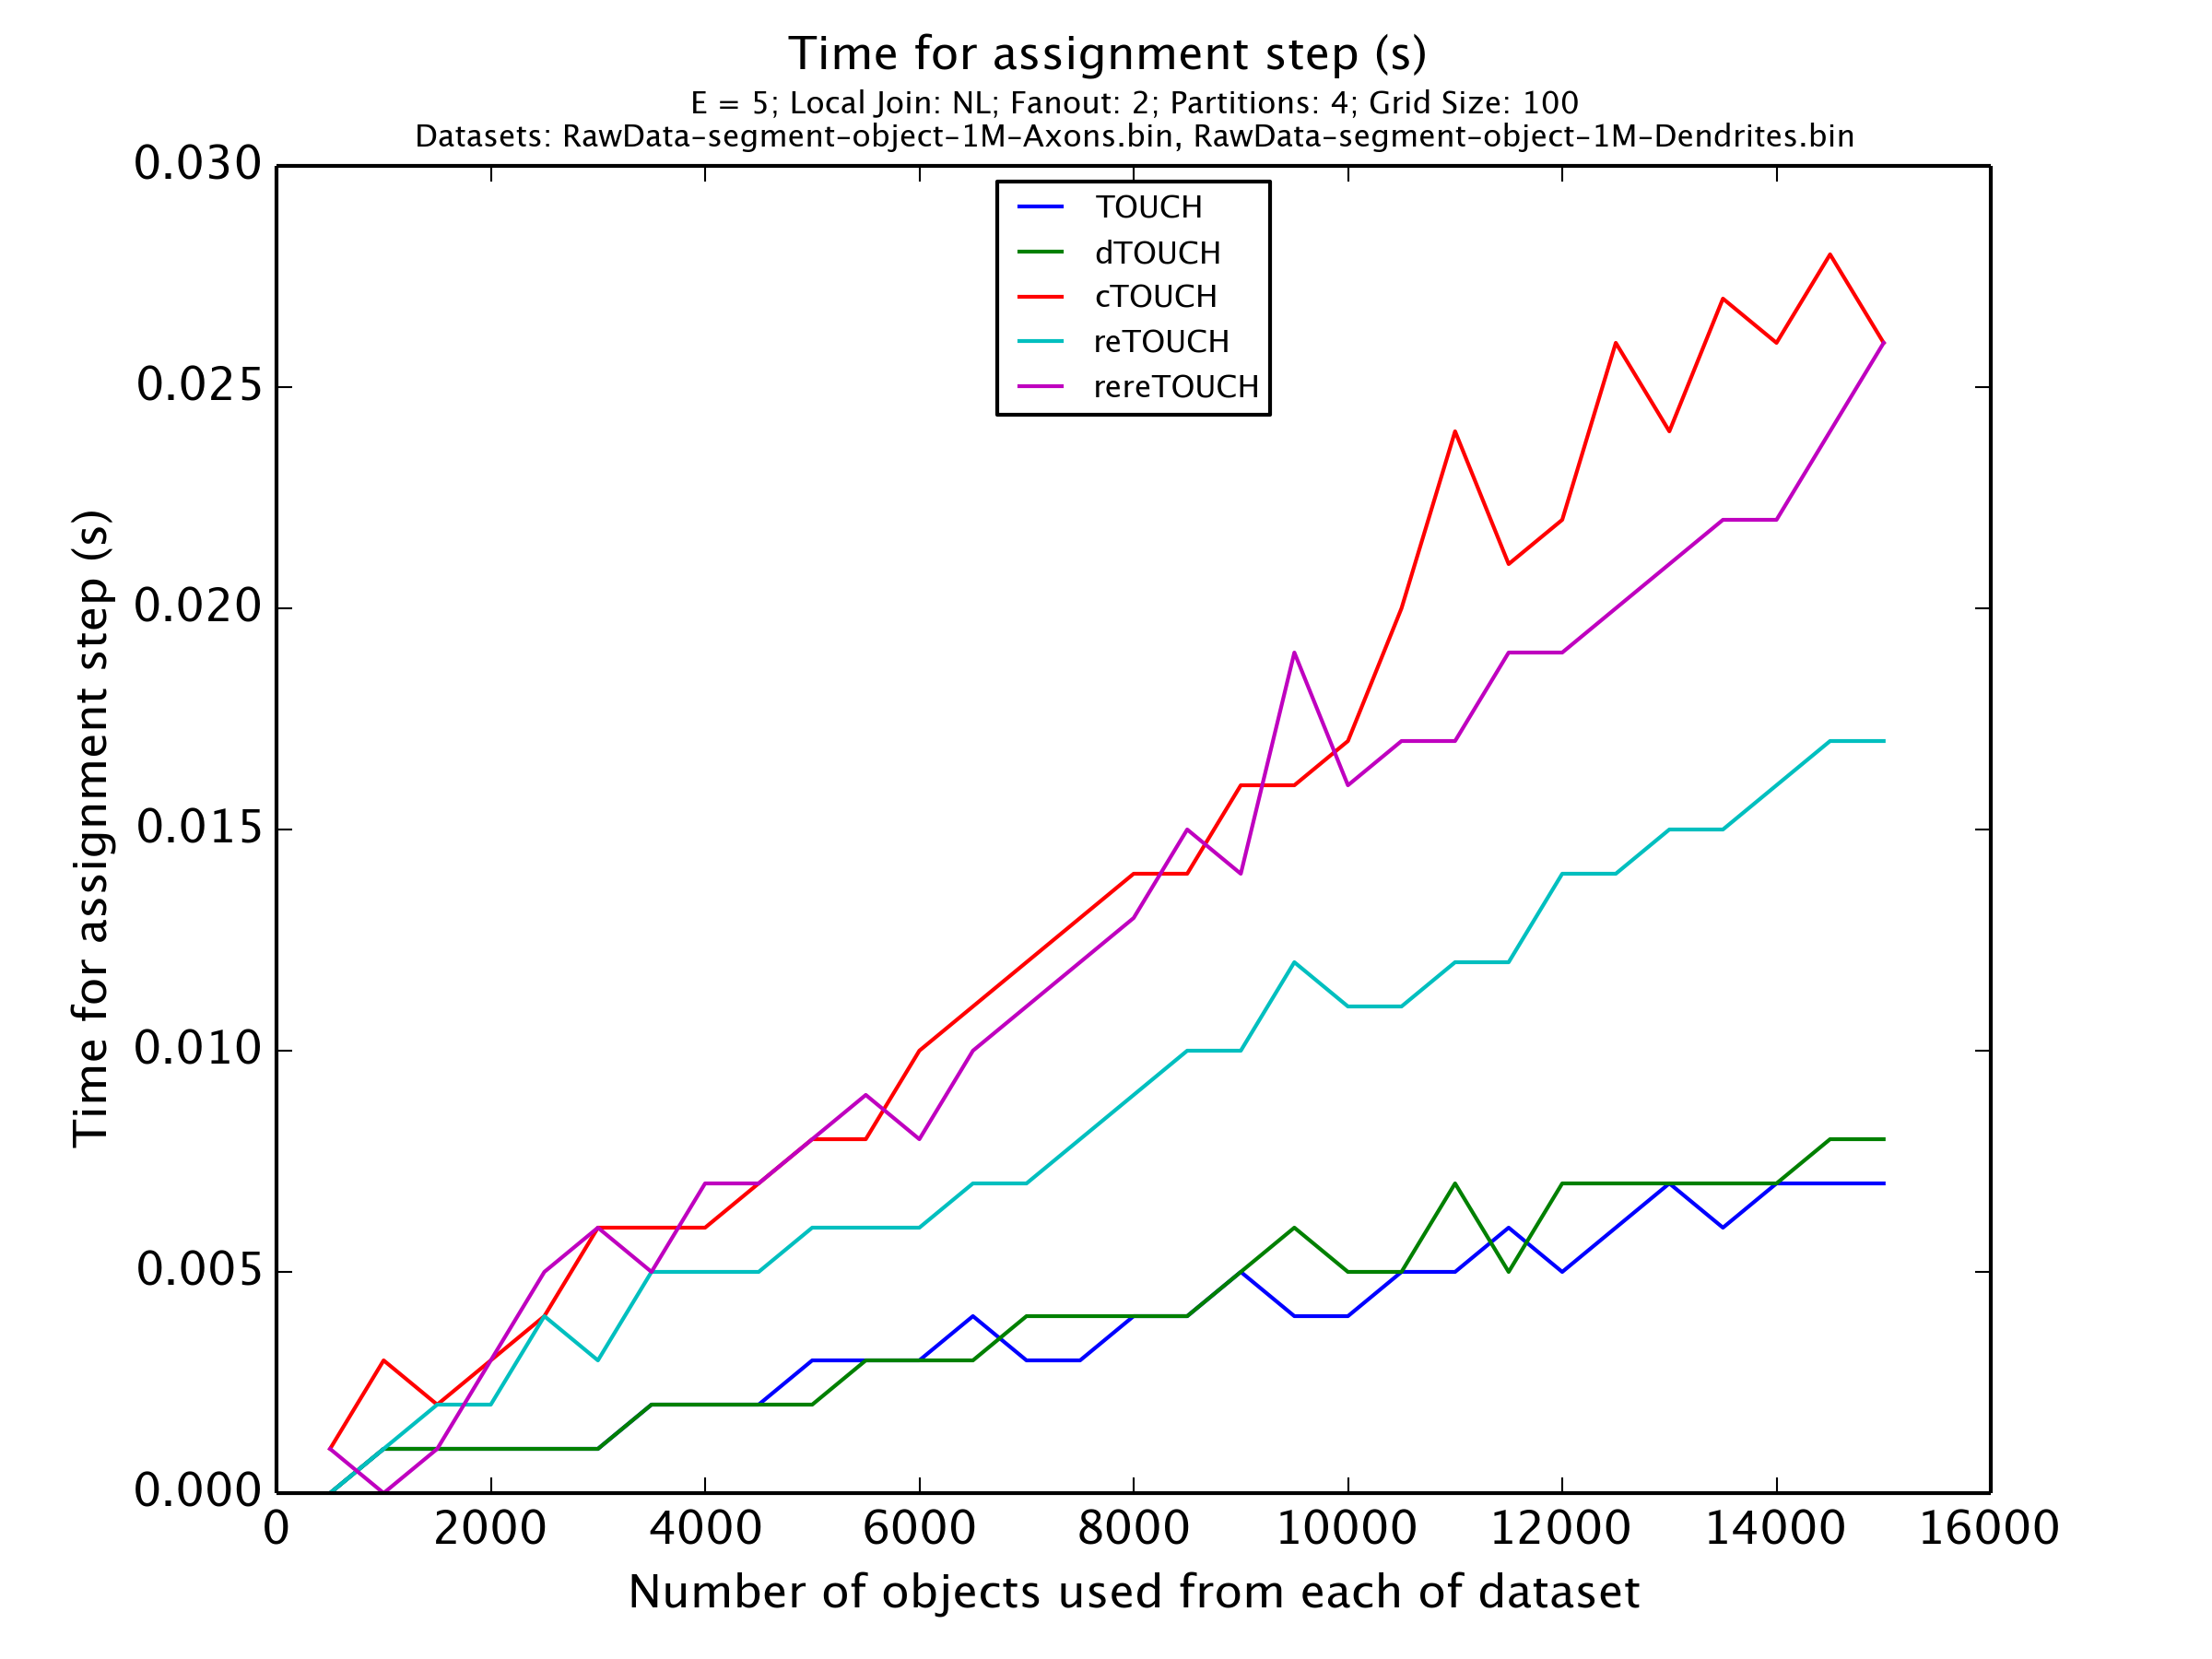
\includegraphics[width=0.8\textwidth]{Images/pic20.png}
\end{figure}
\end{frame}
\begin{frame}{Computational experiment : Join time}
\begin{figure}[p]
    \centering
    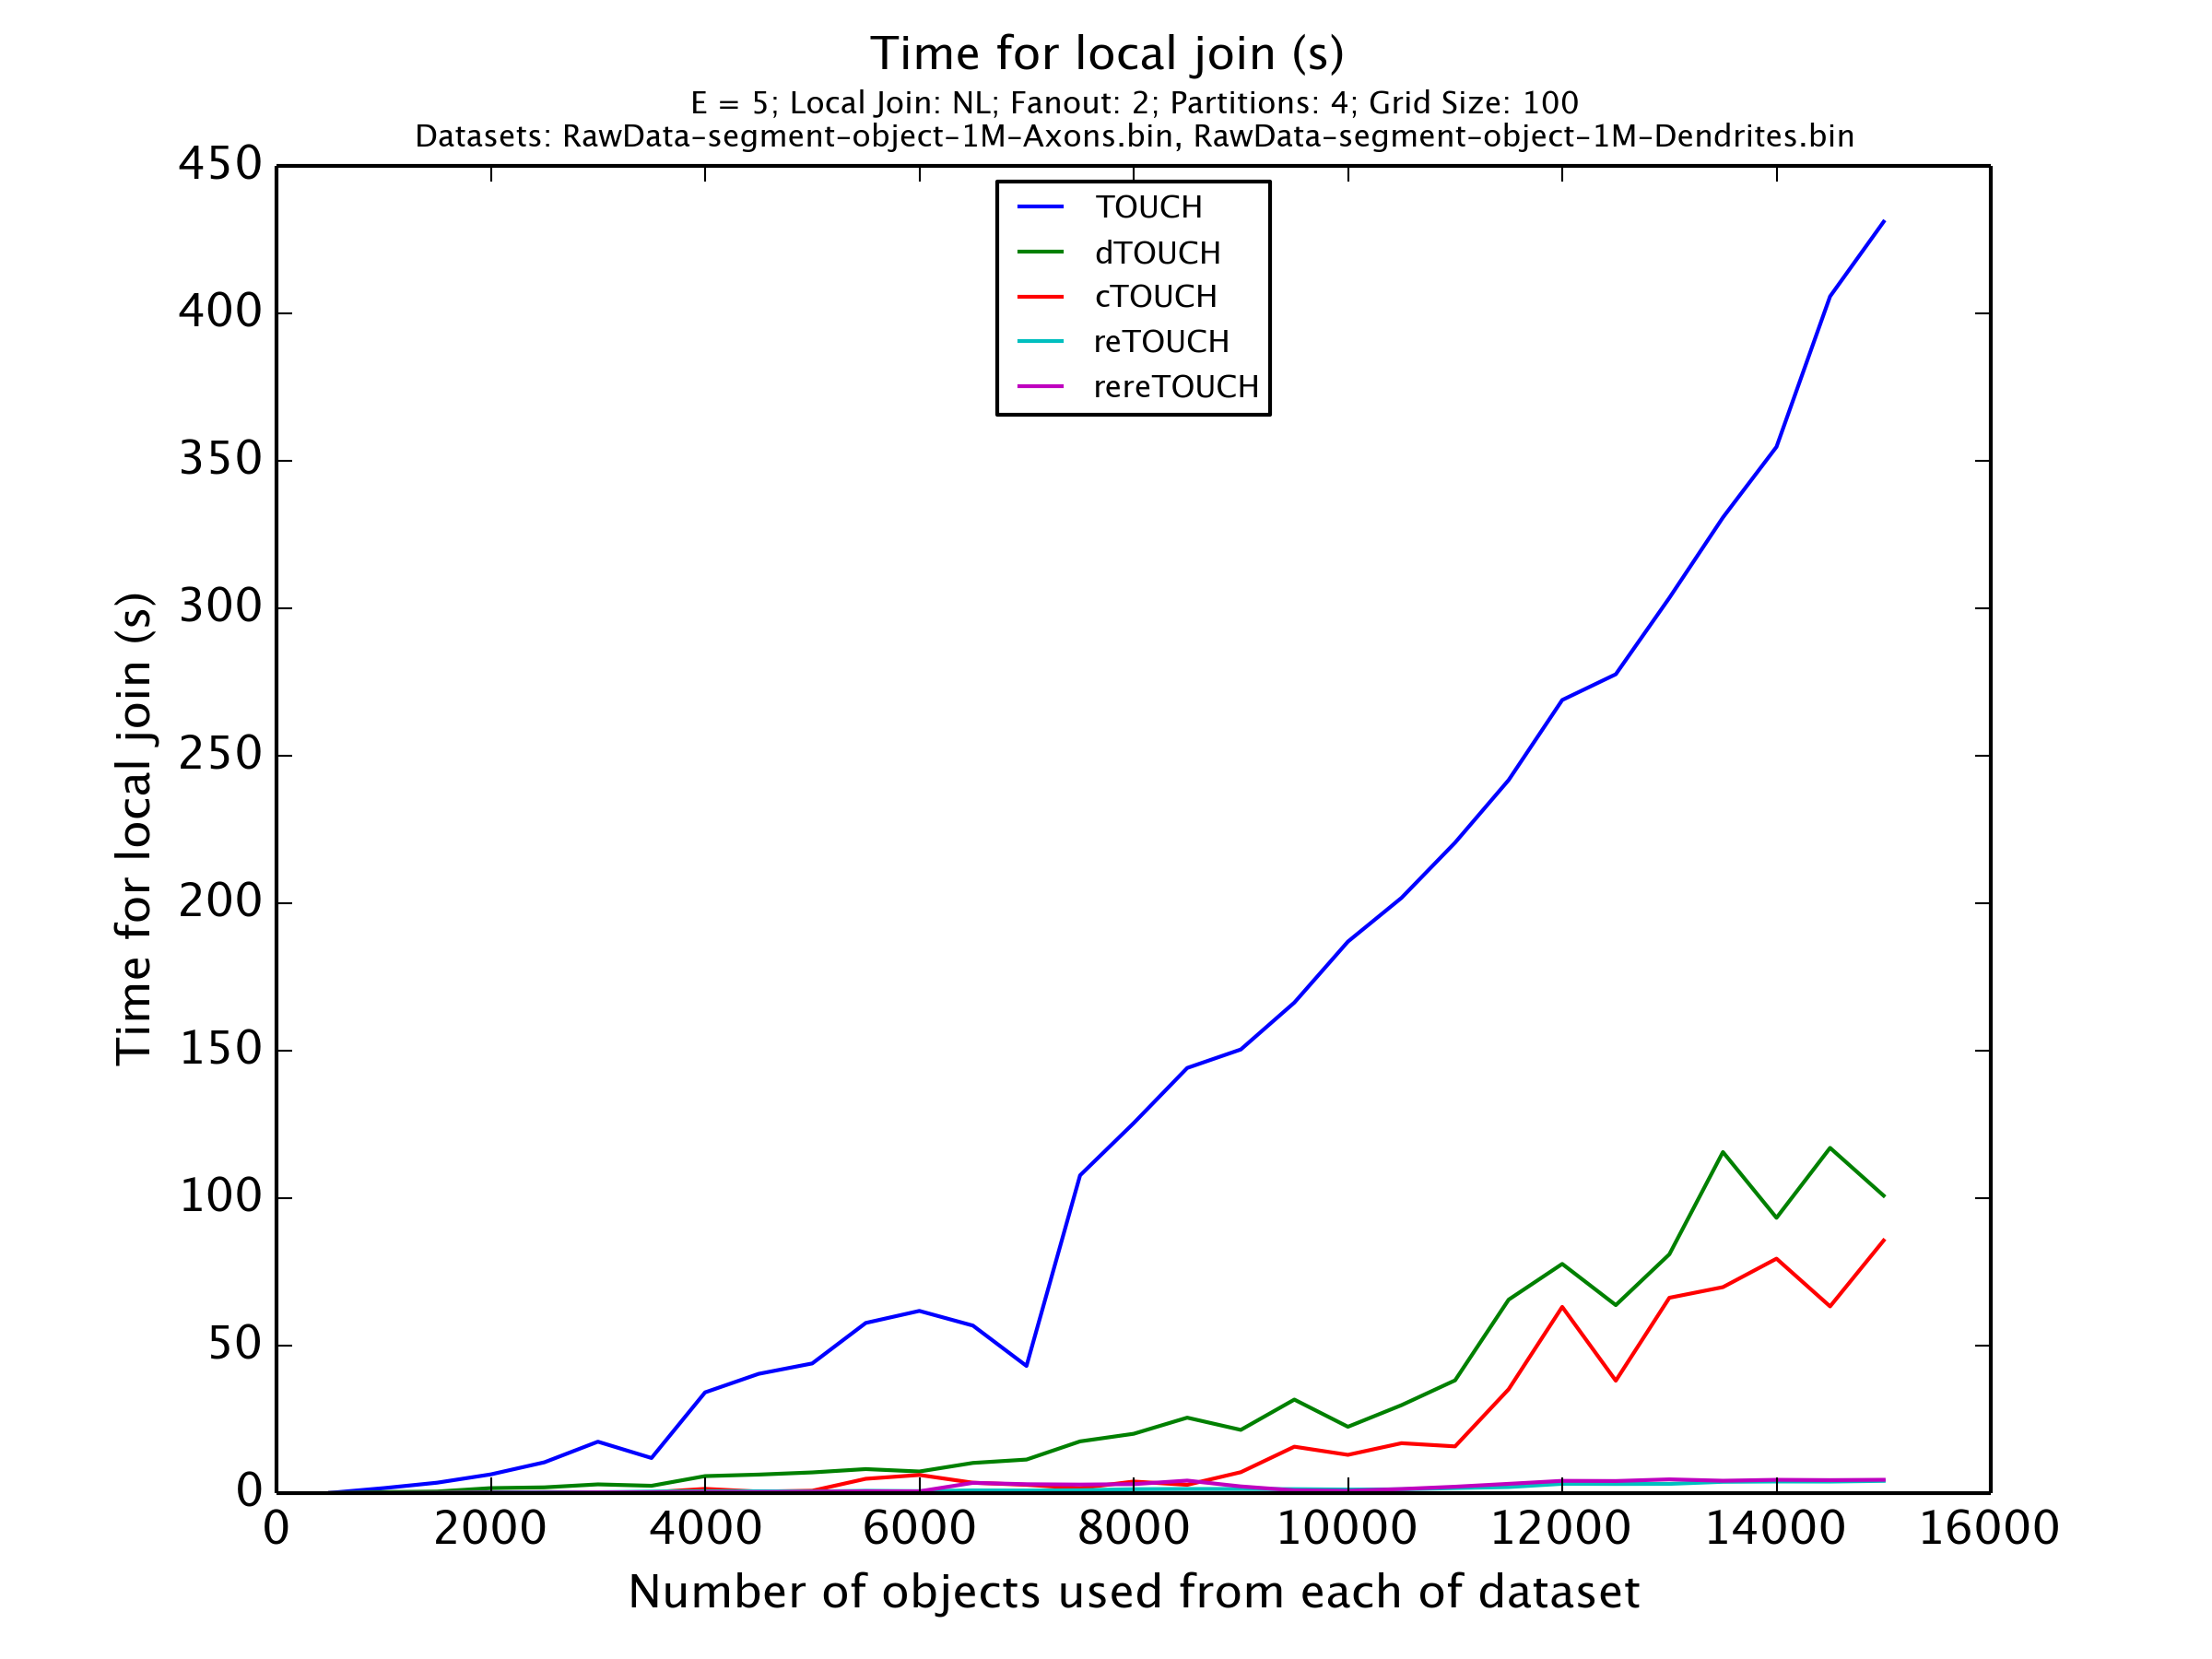
\includegraphics[width=0.8\textwidth]{Images/pic22.png}
\end{figure}
\end{frame}
%----------------------------------------------------------------------------------------------------------
\begin{frame}{Conclusion}
All modifications considerably improve total spatial join time by increasing number of filtered objects and decreasing number of objects that should be checked for intersection.
\end{frame}
%----------------------------------------------------------------------------------------------------------
\end{document} 